\documentclass[11pt]{article}
\usepackage{graphicx}
\usepackage{xcolor}
\usepackage{pagecolor}
\usepackage{afterpage}
\usepackage{transparent}
\usepackage{tikz}
\usepackage{mathptmx}
\usetikzlibrary{shapes.geometric, arrows}
\usepackage[a4paper, total={8in, 10in}]{geometry}
\usepackage{tikz}
\usetikzlibrary{shapes.geometric, arrows}
\usetikzlibrary {shapes.misc}
\definecolor{orange}{HTML}{FB650A}
\definecolor{green}{HTML}{7EFDAA}
\definecolor{yellow}{HTML}{F9DC74}
\definecolor{lblue}{HTML}{82F6EE}
\definecolor{lgreen}{HTML}{F4EF1C}


\tikzstyle{startstop} = [rectangle, rounded corners, 
minimum width=3cm, 
minimum height=1cm,
rounded corners,
text centered, 
% draw=black, 
fill=lblue!100]

\tikzstyle{ev} = [trapezium, 
trapezium stretches=true, % A later addition
trapezium left angle=70, 
trapezium right angle=110, 
minimum width=3cm, 
minimum height=1cm, text centered, 
rounded corners,
% draw=black,
fill=lgreen!100]

\tikzstyle{process} = [rectangle, 
minimum width=3cm, 
minimum height=1cm, 
text centered, 
text width=3cm, 
rounded corners,
% draw=black, 
fill=green!100]

\tikzstyle{decision} = [diamond, 
minimum width=3cm, 
minimum height=1cm,
text centered, 
text width=3cm,
text height=-1cm,
rounded corners,
% draw=black, 
fill=orange!100]
\tikzstyle{arrow} = [thick,->,>=stealth]

\tikzstyle{rounded} = [rounded rectangle, 
minimum width=20cm, 
minimum height=1.7cm,
fill=yellow!100]


\begin{document}






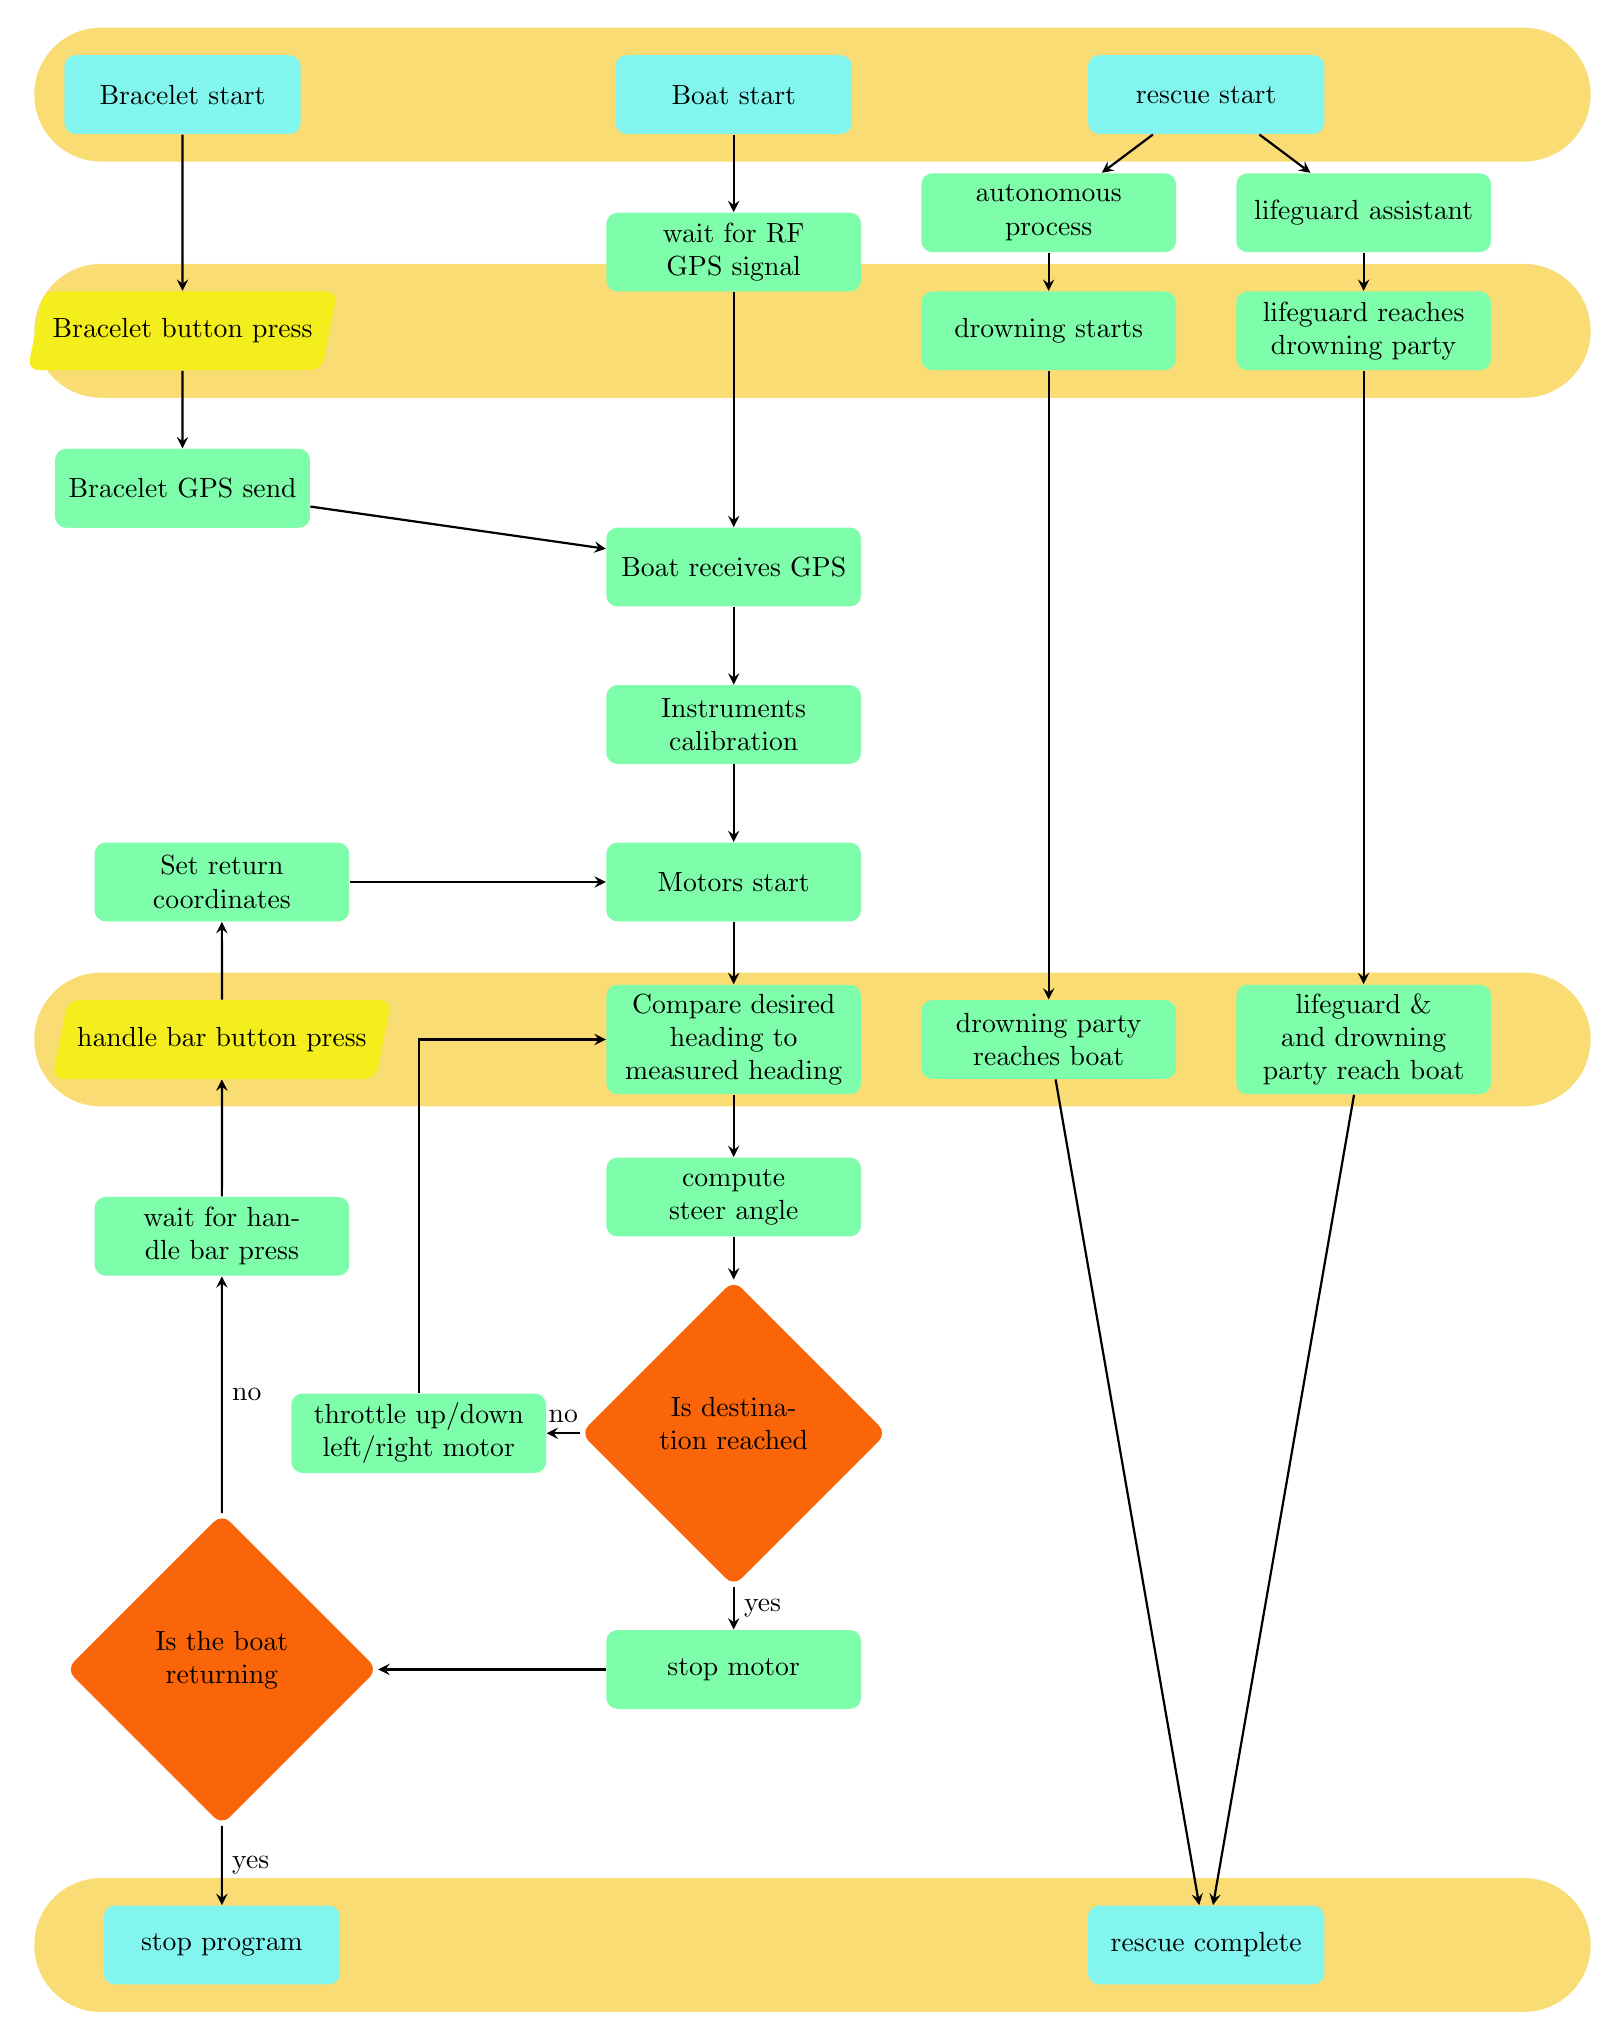
\begin{tikzpicture}[node distance=2cm]
\node (event1) [rounded, xshift=6cm]{};
\node (event1) [rounded, yshift=-3cm, xshift=6cm]{};
\node (event3) [rounded, yshift=-12cm, xshift=6cm]{};
\node (event4) [rounded, yshift=-23.5cm, xshift=6cm]{};
\node (start) [startstop, xshift=-2cm] {Bracelet start};
\node (startb) [startstop, xshift=5cm] {Boat start};
\node (startr) [startstop, xshift=11cm] {rescue start};
\node (ev1) [ev, below of=start, yshift=-1cm] {Bracelet button press};
\node (pro1) [process, below of=ev1] {Bracelet GPS send};
\node (pro2) [process, below of=startb] {wait for RF GPS signal};
\node (pro3) [process, below of=pro2, yshift=-2cm] {Boat receives GPS};
\node (pro4) [process, below of=pro3] {Instruments calibration};
\node (pro5) [process, below of=pro4] {Motors start};
\node (pro6) [process, below of=pro5] {Compare desired heading to measured heading};
\node (pro7) [process, below of=pro6] {compute steer angle};
\node (dec1) [decision, below of=pro7, yshift=-1cm] {Is destination reached};
\node (pro8) [process, below of=pro7, xshift=-4cm, yshift=-1cm] {throttle up/down left/right motor};
\node (pro9) [process, below of=dec1, yshift=-1cm] {stop motor};
\node (pro10) [process, left of=pro8, xshift=-0.5cm, yshift=2.5cm] {wait for handle bar press};
\node (pro11) [startstop, below of=pro10, yshift=-7cm] {stop program};
\node (dec2) [decision, below of=pro8, xshift=-2.5cm, yshift=-1cm] {Is the boat returning};
\node (pro12) [process, left of=pro6, yshift=2cm, xshift=-4.5cm] {Set return coordinates};
\node (ev2) [ev, above of=pro10, yshift=0.5cm] {handle bar button press};
\node (pro1) [process, below of=ev1] {Bracelet GPS send};
\node (pro13) [process, below of=startr, xshift=-2cm, yshift=0.5cm] {autonomous process};
\node (pro14) [process, below of=startr, xshift=2cm, yshift=0.5cm] {lifeguard assistant};
\node (pro15) [process, below of=pro13, yshift=0.5cm] {drowning starts};
\node (pro16) [process, below of=pro14, yshift=0.5cm] {lifeguard reaches drowning party};
\node (pro17) [process, below of=pro15, yshift=-7cm] {drowning party reaches boat};
\node (pro18) [process, below of=pro16, yshift=-7cm] {lifeguard \& and drowning party reach boat};
\node (pro19) [startstop, below of=startr, yshift=-21.5cm] {rescue complete};
% \node (stop) [startstop, below of=out1] {Stop};



\draw [arrow] (start) -- (ev1);
\draw [arrow] (startb) -- (pro2);
\draw [arrow] (ev1) -- (pro1);
\draw[arrow] (pro2) -- (pro3);
\draw [arrow] (pro1) -- (pro3);
\draw[arrow] (pro3) -- (pro4);
\draw[arrow] (pro4) -- (pro5);
\draw[arrow] (pro5) -- (pro6);
\draw [arrow] (pro6) --  (pro7) ;
\draw[arrow] (pro7) -- (dec1);
\draw[arrow] (dec1) -- node[anchor=west] {yes}(pro9);
\draw [arrow] (dec1) -- node[anchor=south] {no} (pro8);
\draw [arrow] (pro8) |- (pro6);
\draw[arrow] (pro9) -- (dec2);
\draw[arrow] (dec2) -- node[anchor=west] {yes}(pro11);
\draw[arrow] (dec2) -- node[anchor=west] {no}(pro10);
\draw[arrow] (pro10) -- (ev2);
\draw[arrow] (ev2) -- (pro12);
\draw[arrow] (pro12) -- (pro5);
\draw[arrow] (startr) -- (pro13);
\draw[arrow] (startr) -- (pro14);
\draw[arrow] (pro13) -- (pro15);
\draw[arrow] (pro14) -- (pro16);
\draw[arrow] (pro15) -- (pro17);
\draw[arrow] (pro16) -- (pro18);
\draw[arrow] (pro18) -- (pro19);
\draw[arrow] (pro17) -- (pro19);



% \draw [arrow,red] (pro10)  -| (pro6);
% \draw [arrow] (pro2a) -- (out1);
% \draw [arrow] (out1) -- (stop);

\end{tikzpicture}
\end{document}